\section{\rm EEG \mc データ}
実験データとしてBCI2000システムを用いて記録された
PhysioNetが提供する運動想起データセットを用いた。
電極の配置は標準的な10-10システム(図\ref{fig:10system})であり、サンプリング周波数は160Hzである。
109人の被験者が定められたタイムスケジュールに従い、
左手、右手、両手および両足の運動想起を行っている。
運動想起のタイムスケジュールを表す図を図\ref{fig:motorimage}に示す。
運動想起の開始時には被験者の前面に配置されたディスプレイから
右手あるいは左手の運動想起の指示が出される。
被験者は4秒間指示された手の
指を開いたり閉じたりする運動想起試行を続け、その後4.2秒間の休息時間が与えられる。
休息時間を終えると再びディスプレイから両手あるいは両足の運動想起の指示が出され、
被験者は4秒間の支持された部位の指を開いたり閉じたりする運動想起試行を行う。その後4.2秒の休息時間が再び与えられる。
計16.4秒を1サイクルとし、被験者1人につき45サイクルを繰り返し行う。
従って被験者は左手、右手、両手、両足で計90回の運動想起を行っている。
\begin{figure}[t]
    \centering
    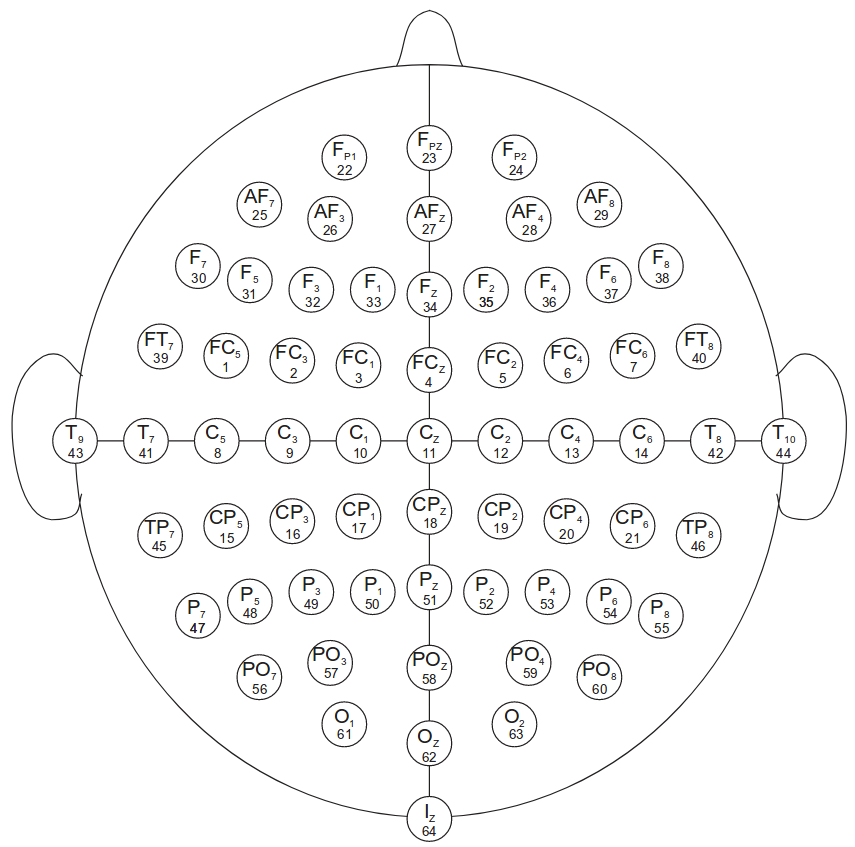
\includegraphics[width=14cm]{images/system1010.png}
    \caption{10-10システムの電極配置}
    \label{fig:10system}
\end{figure}
\begin{figure}[t]
    \centering
    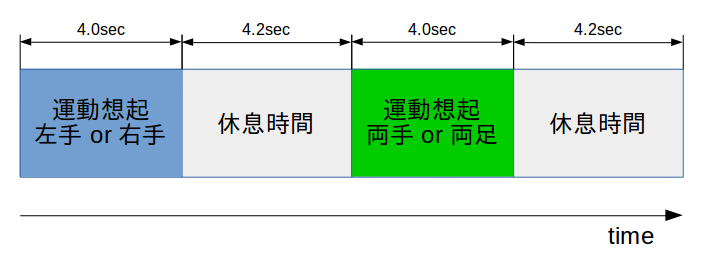
\includegraphics[width=12cm]{images/motorimage.png}
    \caption{運動想起EEG測定のタイムスケジュール}
    \label{fig:motorimage}
\end{figure}
本研究では各運動想起時間である4秒間のデータを取り出して、
2クラス分類の問題を\(_4C_2=6\)種類準備した。
また、以降2クラス分類の問題は表\ref{table:pattern}に示す通り表記する。
\begin{table}[t]
    \centering
    \caption{分類問題の種類と論文内の表記}
    \begin{tabular}{|c|c|} \hline
        分類問題 & 論文内の表記 \\ \hline
        左手or右手 & LR \\ \hline
        両手or両足 & HF \\ \hline
        左手or両手 & LH \\ \hline
        左手or両足 & LF \\ \hline
        右手or両手 & RH \\ \hline
        右手or両足 & RF \\ \hline
    \end{tabular}
    \label{table:pattern}
\end{table}

\subsection{評価方法}
評価方法は正解率とする。
被験者は99人とし、それぞれ6つの分類問題が準備されているため計594の
正解率が得られる。
ある被験者iに関する6つの分類問題の正解率の平均を取ることで、被験者iに対する
BCIの評価を行う。
また、ある分類問題jに関する99人の被験者の正解率の平均を取ることで、分類問題jに対する
BCIの評価を行う。